\documentclass[12pt]{article}
\usepackage[T1]{fontenc}
\usepackage[utf8]{inputenc}
\usepackage[polish]{babel}
\usepackage{lmodern}
\usepackage[a4paper,margin=2.4cm]{geometry}
\usepackage{xcolor}
\usepackage{graphicx}
\usepackage{amsmath,amssymb}
\usepackage{booktabs}
\usepackage{array}
\usepackage{enumitem}
\usepackage{hyperref}
\usepackage{tcolorbox}
\usepackage{fancyhdr}
\definecolor{WEIIPrimary}{RGB}{0,130,150}
\definecolor{WEIIPrimaryDark}{RGB}{0,86,100}
\definecolor{WEIIPrimaryLight}{RGB}{229,246,248}
\definecolor{PRzNavy}{RGB}{31,63,142}
\definecolor{RLTextDark}{RGB}{34,34,34}
\definecolor{RLGray}{RGB}{90,90,90}
\definecolor{RLLightGray}{RGB}{245,246,248}
\definecolor{RLWarning}{RGB}{184,86,0}
\definecolor{RLExample}{RGB}{52,112,64}
\definecolor{RLCodeBg}{RGB}{248,248,248}

\usepackage{listings}
\usepackage{xcolor}

\lstdefinestyle{rlpython}{%
    language=Python,
    basicstyle=\ttfamily\scriptsize,
    keywordstyle=\color{WEIIPrimaryDark}\bfseries,
    commentstyle=\color{RLGray}\itshape,
    stringstyle=\color{RLExample},
    numbers=left,
    numberstyle=\tiny\color{RLGray},
    numbersep=6pt,
    showstringspaces=false,
    breaklines=true,
    tabsize=4,
    frame=single,
    rulecolor=\color{WEIIPrimary!35},
    backgroundcolor=\color{RLCodeBg},
    captionpos=b
}

\lstset{style=rlpython}


\hypersetup{colorlinks=true,linkcolor=WEIIPrimaryDark,urlcolor=WEIIPrimaryDark,citecolor=WEIIPrimaryDark}
\setlength{\headheight}{15pt}
\pagestyle{fancy}
\fancyhf{}
\lhead{Uczenie się ze wzmocnieniem}
\rhead{WEiI PRz}
\cfoot{\thepage}

\newtcolorbox{taskbox}[1]{colback=WEIIPrimaryLight,colframe=WEIIPrimary,title=\textbf{#1}}
\newtcolorbox{notebox}[1]{colback=RLLightGray,colframe=RLGray,title=\textbf{#1}}
\newtcolorbox{warninghandout}[1]{colback=RLWarning!8,colframe=RLWarning,title=\textbf{#1}}

\newcommand{\handouttitle}[3]{%
\begin{center}
{\Large\bfseries #1}\\[0.2cm]
{\large #2}\\[0.15cm]
{\small #3}
\end{center}
\vspace{0.4cm}
\hrule
\vspace{0.6cm}
}

\newcommand{\EnableLabNumbering}{%
  \renewcommand{\thesection}{L\arabic{section}}%
  \renewcommand{\thesubsection}{\thesection.\arabic{subsection}}%
  \renewcommand{\thesubsubsection}{\thesubsection.\arabic{subsubsection}}%
}


\title{Raport projektowy\\Uczenie się ze wzmocnieniem\\[0.35em]\large Dokumentacja projektu -- etapy E1 i E2}
\author{\textbf{Alan Kyciński}}
\date{Rok akademicki 2026/2027}

\begin{document}
\maketitle
\tableofcontents
\newpage


\section{Informacje podstawowe}

\begin{center}
\renewcommand{\arraystretch}{1.22}
\begin{tabular}{p{0.34\textwidth}p{0.56\textwidth}}
\toprule
Element & Informacja \\
\midrule
Imię i nazwisko & \textbf{Alan Kyciński} \\
Numer albumu & \textbf{179545} \\
Kierunek/specjalność & Informatyka / Sztuczna inteligencja \\
Tytuł projektu & Optymalizacja procesu kontroli jakości produktów przemysłowych z wykorzystaniem algorytmu Q-learning \\
Link do repozytorium & {\small\url{https://github.com/KciamiK/DefectDecision-RL}} \\
Data propozycji E1 & \textbf{6 listopada 2026 r.} \\
\bottomrule
\end{tabular}
\end{center}

\section{Temat i cel projektu}

\subsection{Opis problemu}

Projekt \textbf{DefectDecision-RL} dotyczy optymalizacji procesu przemysłowej kontroli jakości z wykorzystaniem uczenia się ze wzmocnieniem. Kontrolowanym wyrobem jest \textbf{prostokątna płytka aluminiowa z czterema otworami montażowymi}. Kolejne płytki mogą być prawidłowe, posiadać dopuszczalne ślady obróbki lub uszkodzenia przekraczające ustalone wymagania jakościowe. Zadaniem systemu jest podejmowanie decyzji dotyczących dalszego postępowania z kontrolowanymi produktami.

Rozważane są \textbf{cztery grupy nieprawidłowości}: (1) rysy powierzchniowe, (2) pęknięcia, (3) nieprawidłowe otwory montażowe oraz (4) plamy i ślady korozji. Na jednej płytce może występować kilka nieprawidłowości jednocześnie. Nie każda z nich oznacza jednak wadliwy produkt. Drobne zarysowania, niewielkie przebarwienia czy odchylenia położenia otworów mogą mieścić się w przyjętych tolerancjach. Natomiast rzeczywiste pęknięcia, brak otworu lub przekroczenie dopuszczalnych odchyleń powodują uznanie produktu za wadliwy. Wszystkie kryteria jakościowe zostaną określone na potrzeby symulacji i nie będą stanowiły rzeczywistych norm przemysłowych.

W środowisku generowane będą \textbf{syntetyczne obrazy 2D płytek} uwzględniające różne rodzaje i stopnie nasilenia uszkodzeń, a także zmienność oświetlenia, faktury powierzchni i szum obrazu. Każdy produkt zostanie poddany wstępnemu skanowaniu, którego wynikiem będzie oszacowanie ryzyka wystąpienia niedopuszczalnej wady. Na podstawie otrzymanych informacji agent wybierze jedną z trzech akcji: \texttt{ACCEPT} (akceptacja), \texttt{REJECT} (odrzucenie) lub \texttt{INSPECT} (dodatkowa kontrola). Szczegółowe badanie dostarczy dokładniejszych informacji, jednak jego wykonanie będzie związane z ograniczonym budżetem inspekcji.

\textbf{Głównym celem projektu jest opracowanie i zbadanie strategii decyzyjnej opartej na algorytmie Q-learning.} Agent będzie uczył się podejmowania decyzji w warunkach niepewności, uwzględniając skuteczność kontroli oraz konsekwencje wykorzystania dostępnych zasobów. Opracowane rozwiązanie zostanie poddane eksperymentom pozwalającym ocenić jego zdolność do ograniczania liczby błędnych decyzji i kosztów inspekcji. Uzyskane wyniki zostaną porównane z rezultatami prostych strategii bazowych.

\subsection{Cel agenta}

Agent ma nauczyć się \textbf{dobierać decyzję do niepewnego wyniku badania, liczby pozostałych płytek i budżetu szczegółowych kontroli}. Celem jest maksymalizacja sumy nagród w całej partii, a nie uzyskanie jak największej liczby pozytywnych wskazań skanera. System powinien:
\begin{itemize}[nosep]
    \item skutecznie identyfikować płytki przekraczające tolerancje jakościowe;
    \item nie odrzucać bez potrzeby płytek z dopuszczalnymi śladami produkcji;
    \item ograniczać koszt dodatkowych badań i zachowywać budżet na kolejne przypadki;
    \item podejmować rozsądne decyzje również przy niejednoznacznych pomiarach.
\end{itemize}

Wyniki oceny będą obejmować średnią nagrodę na partię, udział przeoczonych wad, udział błędnych odrzuceń i liczbę wykonanych badań szczegółowych. Agent Q-learning zostanie porównany z agentem losowym i heurystyką opartą na progach ryzyka. Interfejs w Pygame pokaże produkt, wynik skanu, decyzję agenta, stan budżetu oraz przebieg uczenia i porównania.

\subsection{Uzasadnienie zastosowania uczenia się ze wzmocnieniem}

Problem jest \textbf{sekwencyjny}: w ramach jednej partii agent kontroluje kolejne produkty, a po zleceniu badania szczegółowego może podjąć następną decyzję dotyczącą tej samej płytki. Decyzja o inspekcji wpływa na przyszły stan środowiska, ponieważ zmniejsza budżet pozostały dla kolejnych wyrobów. Decyzje akceptacji i odrzucenia są ostateczne, a ocena skanera bywa niepewna.

Występuje zatem \textbf{konflikt celów}: ograniczenie błędów jakościowych wymaga czasem dodatkowej analizy, ale zasoby na taką analizę są ograniczone. Prosty klasyfikator działający niezależnie dla każdej płytki nie uwzględnia kosztu utraconej możliwości kontroli w przyszłości. Q-learning będzie uczył się strategii maksymalizującej \textbf{długoterminowy zwrot} poprzez wielokrotne epizody i informację zwrotną w postaci nagród i kar. Porównanie z heurystyką pozwoli sprawdzić, czy uczenie jest uzasadnione również praktycznie.

\section{Formalizacja problemu RL/MDP}

\subsection{Agent i środowisko}

\textbf{Agent}: dyskretny kontroler inspekcji, który wybiera działanie dla aktualnej płytki na podstawie obserwowanych wyników badań i pozostałego budżetu.

\textbf{Środowisko}: autorski symulator generujący płytki 2D, ich ukrytą zgodność z wymaganiami, wyniki skanowania i nagrody. Generator przechowuje rzeczywiste parametry defektów (np. geometrię rysy i otworów), a reguły tolerancji wyznaczają etykietę \(y\in\{0,1\}\), gdzie \(0\) oznacza płytkę zgodną z wymaganiami, a \(1\) -- wadliwą. \textbf{Etykieta \(y\) nie jest przekazywana agentowi przed końcową decyzją}. Używa jej środowisko do naliczenia nagrody.

Każdy krok realizuje interfejs \texttt{reset()} oraz \texttt{step(action)}. Po \texttt{ACCEPT} albo \texttt{REJECT} środowisko rozlicza decyzję i przechodzi do następnej płytki. Po \texttt{INSPECT} zużywa jedną kontrolę, udostępnia dodatkowy, niedoskonały wynik skanera i pozostaje przy tym samym produkcie. Skanery nie wykonują za agenta decyzji końcowej.

\subsection{Stan lub obserwacja}

Pełny stan środowiska zawiera m.in. ukryte parametry defektów i faktyczną zgodność płytki. Agent otrzymuje wyłącznie \textbf{dyskretną obserwację}:
\begin{equation}
    s_t=(n_t,b_t,w_t,z_t),
\end{equation}
\noindent gdzie:
\begin{center}
\renewcommand{\arraystretch}{1.2}
\begin{tabular}{p{0.29\textwidth}p{0.61\textwidth}}
\toprule
Składowa & Znaczenie \\
\midrule
\(n_t\in\{1,\ldots,10\}\) & Liczba płytek do rozstrzygnięcia, wliczając bieżącą. \\
\(b_t\in\{0,\ldots,4\}\) & Pozostała liczba badań szczegółowych w partii. \\
\(w_t\in\{L,M,H\}\) & Niska, średnia lub wysoka kategoria ryzyka po skanie podstawowym. \\
\(z_t\in\{\varnothing,-,+\}\) & Brak dodatkowego badania albo jego wynik: brak wskazania wady / wskazanie wady. \\
\bottomrule
\end{tabular}
\end{center}

Przykład \(s=(7,3,M,\varnothing)\) oznacza siedem płytek pozostałych do decyzji, trzy dodatkowe kontrole i średnie ryzyko dla płytki dotychczas badanej tylko podstawowo. Wariant \(z\neq\varnothing\) sygnalizuje, że dodatkowy skan już wykonano. Pełne wyniki czterech analizowanych cech będą widoczne w panelu informacyjnym, natomiast \textbf{do tablicy Q trafi ich zwięzłe podsumowanie}. Utrzymuje to niewielką przestrzeń stanów.

W formalnym ujęciu jakość produktu jest częściowo obserwowalna (problem zbliżony do POMDP). Używana obserwacja \(s_t\) będzie \textbf{przybliżeniem stanu decyzyjnego}, opartym na skategoryzowanych wynikach badań i zasobach. Przy stałych parametrach symulacji posłuży do tablicowego Q-learningu, a ograniczenie wynikające z utraty szczegółów pomiaru zostanie omówione w raporcie. Tabela przechowuje maksymalnie \(10\cdot5\cdot3\cdot3\cdot3=1350\) wartości \(Q(s,a)\), z których część odpowiada niedozwolonym lub nieosiągalnym przypadkom.

\subsection{Akcje}

\begin{center}
\renewcommand{\arraystretch}{1.22}
\begin{tabular}{p{0.28\textwidth}p{0.62\textwidth}}
\toprule
Akcja & Działanie i następstwa \\
\midrule
\(a=0\), \texttt{ACCEPT} & Przyjęcie płytki; nagroda za zgodną z prawdą decyzję albo kara za przeoczenie wady; przejście do następnej płytki. \\
\(a=1\), \texttt{REJECT} & Odrzucenie płytki; nagroda za wykrycie wady albo kara za odrzucenie prawidłowego wyrobu; przejście do następnej płytki. \\
\(a=2\), \texttt{INSPECT} & Dodatkowy skan bieżącej płytki, zużycie jednostki budżetu, nowy wynik badania i ponowny wybór decyzji. \\
\bottomrule
\end{tabular}
\end{center}

Akcja \texttt{INSPECT} jest \textbf{niedostępna}, gdy \(b_t=0\) lub \(z_t\neq\varnothing\), czyli płytka została już sprawdzona dodatkowo. Nie ma możliwości wykonania więcej niż jednego dodatkowego badania tej samej płytki. Wybór akcji i aktualizacja Q będą uwzględniać wyłącznie legalne działania; pozostałe akcje są zawsze dostępne.

\subsection{Funkcja nagrody}

Środowisko oblicza nagrodę na podstawie wybranej akcji i \textbf{rzeczywistej zgodności z tolerancjami}, a nie na podstawie samego wyniku skanera. Przyjmujemy następujące \textbf{wstępne} wartości:
\begin{equation}
 r_t=\begin{cases}
 +2, & a_t=\mathrm{ACCEPT}\ \land\ y_t=0,\\
 -12, & a_t=\mathrm{ACCEPT}\ \land\ y_t=1,\\
 +5, & a_t=\mathrm{REJECT}\ \land\ y_t=1,\\
 -4, & a_t=\mathrm{REJECT}\ \land\ y_t=0,\\
 -1, & a_t=\mathrm{INSPECT}.
 \end{cases}
\end{equation}

Największa kara \(-12\) dotyczy przepuszczenia wadliwej płytki. Odrzucenie płytki mieszczącej się w tolerancji również jest błędem (kara \(-4\)), nawet gdy ma ona widoczne drobne rysy lub przebarwienia. Inspekcja kosztuje \(-1\), dlatego agent powinien ją wybierać tylko wtedy, gdy wartość dodatkowej informacji uzasadnia koszt teraz i stratę części budżetu na przyszłość. Poprawne rozstrzygnięcia przynoszą nagrodę dodatnią.

Nie wprowadzamy dodatkowej kary za każdy krok. Dopuszczalność akcji i ograniczona liczba inspekcji zapobiegają niekończącym się epizodom. \textbf{Wagi nagród będą badane eksperymentalnie}; możliwe niepożądane strategie, np. zbyt częste odrzucanie produktów, zostaną ocenione osobno przez metryki błędów.

\subsection{Warunki zakończenia epizodu}

\textbf{Jeden epizod to jedna partia 10 aluminiowych płytek}. Na początku epizodu losowana jest nowa partia, a budżet szczegółowych badań wynosi \textbf{4}. Epizod kończy się po podjęciu ostatecznej decyzji \texttt{ACCEPT} albo \texttt{REJECT} dla dziesiątej płytki. Wyczerpanie budżetu nie kończy epizodu: dalsze płytki trzeba rozpatrzyć bez dodatkowego skanowania.

W jednym epizodzie występuje \textbf{10 decyzji końcowych i najwyżej 4 dodatkowe skany}, czyli łącznie od 10 do 14 akcji. Za ostatnią decyzję przyznawana jest normalna nagroda, po czym środowisko zwraca znacznik końca epizodu. Liczba działań jest ograniczona i nie ma ryzyka nieskończonej sekwencji.

\subsection{Założenia i ograniczenia środowiska}

\textbf{Produkt i tolerancje.} W projekcie kontrolowany będzie jeden typ wyrobu: płytka z czterema otworami. Generator tworzy obrazy prawidłowych płytek oraz cztery grupy nieprawidłowości o losowym natężeniu. O etykiecie produktu decydują \textbf{zdefiniowane wcześniej reguły jakościowe}, np. maksymalna wielkość rysy, dopuszczalne odchylenie otworu i zakres przebarwienia. Prawdziwe pęknięcie i brak otworu zawsze oznaczają wadę; drobne ślady obróbki mogą być akceptowalne. Tolerancje służą wyłącznie do zbudowania wiarygodnej symulacji, nie do certyfikowania rzeczywistych części. Możliwe będzie współwystępowanie kilku śladów na jednej płytce.

\textbf{Wyniki skanerów.} Skaner podstawowy oceni w uproszczeniu cztery obszary: linie i rysy, nieregularne pęknięcia, geometrię otworów oraz plamy. Będzie działał na mniej szczegółowym obrazie; skaner dodatkowy skorzysta z dokładniejszego pomiaru. Oba będą obarczone szumem i mogą popełniać błędy. Do analizy 2D przewiduje się proste operacje na obrazie (np. OpenCV), bez trenowania detektora sieciowego. Skaner \textbf{nie otrzyma z generatora informacji o prawdziwych wadach}; analizować będzie tylko obraz. Wstępnie dopuszcza się model statystyczny wyników badań do przetestowania samego środowiska RL, zanim powstanie pełny prosty skaner obrazu.

\textbf{Wynik ryzyka.} Każdy skaner będzie przedstawiał wyniki pomiarów cząstkowych; na ich podstawie zostanie wyznaczony zbiorczy wynik ryzyka. Wyniku nie należy przedstawiać jako rzeczywistego \emph{procentowego prawdopodobieństwa} bez kalibracji. Początkowo będzie to wynik umowny 0--100, a dla Q-learningu zostanie zamieniony na kategorie \(L,M,H\). Jeśli pozwolą na to wyniki testów, oszacowanie prawdopodobieństwa wady będzie kalibrowane na oddzielnym zbiorze syntetycznych przykładów. Do agenta nie trafi prawdziwa etykieta defektu ani informacja o przekroczonych tolerancjach.

\textbf{Ograniczenia i realizacja etapowa.} Model pomija fizyczne własności metalu, rzeczywiste kamery, koszty produkcji oraz złożone defekty przemysłowe. \textbf{Priorytetem jest działający, zweryfikowany agent RL}: (1) generator płytek i etykiet oraz testy środowiska, (2) podstawowy i dodatkowy model obserwacji, (3) agenci losowy, heurystyczny i Q-learning, (4) prosty skaner syntetycznych obrazów, wizualizacja Pygame i eksperymenty. Jeśli etap analizy obrazów okaże się zbyt złożony, będzie uproszczony bez zmiany problemu decyzyjnego i formalizacji RL.

\textbf{Plan uczenia i oceny.} Zostanie zastosowany tablicowy Q-learning z eksploracją \(\varepsilon\)-greedy. Wstępnie przyjmuje się \(\alpha=0{,}1\), \(\gamma=0{,}95\), stopniowe zmniejszanie \(\varepsilon\) od \(1{,}0\) do \(0{,}05\) oraz około 20\,000 epizodów treningowych. Parametry są propozycją, nie ustalonym wynikiem badań. W eksperymentach planuje się porównanie z agentem losowym i regułowym, zmianę budżetu oraz trudności skanowania i analizę liczby przeoczonych wad, błędnych odrzuceń, średniej nagrody i wykorzystania badań. Losowania treningowe i testowe będą rozdzielone, a ziarna losowe zapisane, aby wyniki dało się odtworzyć.


\section{Implementacja}

\noindent\textbf{Stan realizacji: etap E2.}
W niniejszej części przedstawiono elementy \emph{rzeczywiście uruchomione i przetestowane} w etapie E2. Wersja ta wykorzystuje statystyczny model obserwacji zamiast analizy obrazów. Nie zawiera jeszcze wytrenowanego agenta Q-learning ani interfejsu graficznego Pygame.

\subsection{Struktura repozytorium}

Repozytorium \textbf{DefectDecision-RL} zawiera kod Pythona, eksperymenty, testy, wyniki oraz dokumentację. Najważniejsze pliki etapu E2 są uporządkowane w następujący sposób:

\begin{verbatim}
DefectDecision-RL/
|-- src/
|   |-- plate.py
|   |-- plate_generator.py
|   |-- scanner.py
|   |-- detailed_scanner.py
|   |-- quality_env.py
|   |-- random_agent.py
|   `-- heuristic_agent.py
|-- experiments/
|   `-- compare_baselines.py
|-- tests/
|   |-- test_quality_env.py
|   `-- test_env_edge_cases.py
|-- results/
|   |-- baseline_episodes.csv
|   `-- baseline_summary.csv
|-- report/
|-- README.md
|-- requirements.txt
`-- .gitignore
\end{verbatim}

Katalog \texttt{src/} przechowuje klasy domenowe, modele skanerów, środowisko oraz agentów. Skrypty w \texttt{experiments/} wykonują pomiary, \texttt{tests/} zawiera testy jednostkowe, a \texttt{results/} -- wyniki zapisane w formacie CSV. Plik \texttt{requirements.txt} deklaruje zależności środowiska. Katalog \texttt{.venv/} jest lokalny i pomijany przez Git.

\subsection{Model produktu i generator partii}

Klasa \texttt{Plate}, zdefiniowana w \texttt{src/plate.py}, przechowuje numer produktu i natężenie czterech grup nieprawidłowości: rys, pęknięć, wad otworów i korozji. Każda z tych wartości należy do zbioru \(\{0,1,2,3\}\), przy czym zero oznacza brak danej nieprawidłowości. Reguły w metodzie \texttt{is\_defective()} kwalifikują płytkę jako wadliwą, jeżeli wystąpi przynajmniej jeden z warunków:
\begin{itemize}[nosep]
    \item natężenie rys co najmniej 2;
    \item natężenie pęknięć co najmniej 1;
    \item natężenie wady otworów co najmniej 1;
    \item natężenie korozji co najmniej 2.
\end{itemize}

Są to umowne progi demonstracyjnego symulatora, a nie wymagania rzeczywistego zakładu produkcyjnego. W szczególności obecne \texttt{hole\_errors=1} oznacza już niedopuszczalną wadę. Możliwość dopuszczenia bardzo małych odchyłek geometrycznych, sygnalizowana w propozycji E1, zostanie sprecyzowana w kolejnej wersji generatora obrazów.

Funkcja \texttt{generate\_plates()} w \texttt{src/plate\_generator.py} losuje nowe partie; domyślnie partia zawiera dziesięć płytek. Dla każdej cechy użyto osobnego dyskretnego rozkładu z wagami, np. dla rys poziomy 0--3 mają wagi odpowiednio 55\%, 25\%, 15\% i 5\%. Losowanie może otrzymać ustalone ziarno \texttt{seed}, co umożliwia odtworzenie danych eksperymentu.

\subsection{Symulacja skanowania}

Podstawowy skaner \texttt{BasicScanner} działa na rzeczywistych \emph{liczbowych cechach syntetycznej płytki} i zwraca ich niedoskonałe pomiary. Każda z czterech zmiennych jest niezależnie zakłócana z prawdopodobieństwem 0,25; przy zakłóceniu wynik różni się o jeden poziom, pozostając w przedziale 0--3. Skaner \texttt{DetailedScanner} dziedziczy po skanerze podstawowym, lecz stosuje prawdopodobieństwo błędu 0,05.

Procenty 25\% i 5\% oznaczają \emph{parametry modelu pomiarowego dla pojedynczej cechy}, a nie wynik oceny prawidłowości całej płytki. Na obecnym etapie skanery nie przetwarzają pikseli. Ten stan implementacji odpowiada dopuszczonemu w propozycji E1 prototypowi statystycznemu, poprzedzającemu właściwą analizę obrazów 2D.

\subsection{Środowisko decyzyjne}

Środowisko realizuje klasa \texttt{QualityControlEnv}.\par\noindent Jej kod źródłowy znajduje się w pliku \path{src/quality_env.py}. Metoda \texttt{reset()} generuje nową partię, inicjalizuje skanery, ustawia licznik płytek oraz odnawia budżet czterech inspekcji. Metoda \texttt{step(action)} wykonuje legalną akcję i zwraca cztery elementy: nową obserwację, nagrodę, znacznik zakończenia oraz informacje pomocnicze.

Obserwacja jest krotką \(s=(n,b,w,z)\), zgodną z rozdziałem 3. Ryzyko \(w\) wyznacza funkcja \texttt{risk\_category()} na podstawie odczytów podstawowego skanera i umownych punktów dla czterech cech. Wynik jest dzielony na kategorie \(L\), \(M\), \(H\); nie jest to skalibrowane prawdopodobieństwo wady. Po wykonaniu akcji \texttt{INSPECT} zmienna \(z\) przyjmuje wartość \texttt{+} albo \texttt{-}, a liczba dostępnych badań maleje o jeden.

Akcje \texttt{ACCEPT} i \texttt{REJECT} rozliczają produkt według jego rzeczywistej jakości i przechodzą do następnej płytki. Akcja \texttt{INSPECT} nie kończy rozpatrywania bieżącego produktu. Funkcja \texttt{valid\_actions()} zapobiega powtórzeniu inspekcji tej samej płytki oraz wykonaniu jej po wyczerpaniu budżetu. Epizod kończy się po dziesięciu rozstrzygnięciach końcowych; budżet może wyczerpać się wcześniej.

Wykorzystana funkcja nagrody jest zgodna z propozycją E1: \(+2\) za zaakceptowanie produktu poprawnego, \(-12\) za zaakceptowanie wadliwego, \(+5\) za odrzucenie wadliwego, \(-4\) za odrzucenie poprawnego oraz \(-1\) za dodatkową inspekcję. Dzięki temu testowane strategie stają wobec kompromisu między liczbą błędów i kosztem pozyskiwania dokładniejszych informacji.

\subsection{Agenci bazowi}

\textbf{Agent losowy} (\texttt{RandomAgent}, plik \texttt{src/random\_agent.py}) w każdym kroku wybiera jedną z legalnych akcji z jednakowym prawdopodobieństwem. Nie ma dostępu do prawdziwej etykiety płytki i nie aktualizuje żadnej polityki.

\textbf{Agent heurystyczny} (\texttt{HeuristicAgent}, plik \texttt{src/heuristic\_agent.py}) działa na podstawie prostych reguł: dla ryzyka \(L\) akceptuje produkt, dla \(H\) odrzuca go, a dla \(M\) zleca dodatkową kontrolę, jeśli jest dostępna. Gdy budżet się wyczerpie, dla \(M\) wybiera akceptację. Po badaniu szczegółowym akceptuje produkt przy wyniku \texttt{-} i odrzuca przy \texttt{+}. Heurystyka została ustalona przed eksperymentami i nie jest agentem uczącym się.

Agenci korzystają wyłącznie z obserwacji i listy legalnych działań. Rzeczywista jakość produktu służy jedynie do obliczania nagrody i późniejszej ewaluacji.

\subsection{Testy automatyczne}

Poprawność podstawowych mechanizmów sprawdzono biblioteką \texttt{pytest}. Zrealizowano \textbf{18 przypadków testowych}; w ostatnim uruchomieniu wszystkie zakończyły się pomyślnie. Zakres testów obejmuje między innymi inicjalizację i ponowny start epizodu, zgodność zestawu legalnych akcji, ograniczenie budżetu, zakaz podwójnego skanowania, działanie po końcu epizodu, poprawność nagród, konfiguracje brzegowe oraz odtwarzalność dla stałego ziarna losowego.

Zaliczenie testów potwierdza zgodność przebadanych przypadków z założeniami, ale nie zastępuje sprawdzenia jakości strategii na większej próbie ani testów przyszłego skanera obrazu.

\subsection{Agent uczący się -- zakres etapu E3}

Na etapie E2 \textbf{nie zaimplementowano jeszcze tablicowego Q-learningu}. Planowana metoda będzie aktualizowała wartości \(Q(s,a)\), korzystając z nagrody, kolejnej obserwacji oraz legalnych działań. Wartości początkowe i harmonogram \(\varepsilon\)-greedy zostaną określone przed eksperymentami E3; proponowane w E1 parametry mają charakter wstępny. Ta podsekcja zostanie rozbudowana po wdrożeniu algorytmu.

\section{Plan eksperymentów}

\subsection{Eksperyment zrealizowany w E2}

Za pomocą skryptu \texttt{experiments/compare\_baselines.py} porównano agentów losowego i heurystycznego. Każdy z nich przeprowadził \textbf{1000 epizodów}, po dziesięć produktów każdy, czyli łącznie \textbf{20\,000 decyzji końcowych} w dwóch grupach eksperymentalnych. Użyto ziarna nadrzędnego \texttt{SEED=2026}; obaj agenci otrzymali te same 1000 ziaren środowiska, a więc te same wygenerowane partie produktów. Generator losowych decyzji agenta losowego miał oddzielne ziarno.

Wyniki dla pojedynczych epizodów zapisano w \texttt{results/baseline\_episodes.csv}, a agregaty -- w \texttt{results/baseline\_summary.csv}. Zastosowano następujące miary:
\begin{itemize}[nosep]
    \item \textbf{średnia nagroda} -- średnia suma nagród z epizodu;
    \item \textbf{skuteczność} -- liczba poprawnych decyzji końcowych w stosunku do wszystkich decyzji;
    \item \textbf{odsetek przeoczonych wad} -- liczba wadliwych płytek zaakceptowanych w stosunku do wszystkich wadliwych płytek;
    \item \textbf{odsetek błędnych odrzuceń} -- liczba poprawnych płytek odrzuconych w stosunku do wszystkich poprawnych płytek;
    \item \textbf{średnia liczba inspekcji} -- liczba badań dodatkowych na epizod.
\end{itemize}

\subsection{Planowane eksperymenty E3}

\begin{center}
\small
\renewcommand{\arraystretch}{1.2}
\begin{tabular}{p{0.18\textwidth}p{0.38\textwidth}p{0.32\textwidth}}
\toprule
Wariant & Zmienna eksperymentalna & Główne miary \\
\midrule
B1 (E2) & Strategia: losowa lub heurystyczna & Zwrot, skuteczność, błędy, zużycie inspekcji \\
B2 (E3) & Strategia: Q-learning wobec obu bazowych & Te same miary na osobnych epizodach testowych \\
B3 (E3) & Budżet inspekcji i poziom szumu skanerów & Stabilność i wrażliwość polityki na trudność \\
B4 (E3) & Parametry \(\alpha\), \(\gamma\), \(\varepsilon\) i liczba epizodów & Zbieżność, zwrot, zmienność rezultatów \\
\bottomrule
\end{tabular}
\end{center}

W E3 planuje się około 20\,000 epizodów treningowych w wariancie podstawowym, co najmniej kilka niezależnych ziaren treningowych oraz oddzielne zbiory epizodów do oceny końcowej. Szczegółowe wartości hiperparametrów zostaną udokumentowane przy implementacji. Wykres uczenia będzie przygotowany dopiero po rzeczywistym treningu agenta.

\section{Wyniki}

\subsection{Porównanie agentów bazowych w E2}

W tabeli przedstawiono wyniki faktycznie uzyskane dla 1000 epizodów na agenta, odczytane z zapisanych plików CSV.

\begin{center}
\small
\renewcommand{\arraystretch}{1.25}
\begin{tabular}{p{0.46\textwidth}rr}
\toprule
Miara & Agent losowy & Agent heurystyczny \\
\midrule
Średni zwrot na epizod & \(-24{,}873\) & \(+16{,}011\) \\
Skuteczność decyzji & \(50{,}57\%\) & \(73{,}07\%\) \\
Przeoczone wady & \(50{,}21\%\) & \(0{,}87\%\) \\
Błędne odrzucenia & \(48{,}71\%\) & \(51{,}02\%\) \\
Średnia liczba inspekcji & \(3{,}095\) & \(1{,}781\) \\
\bottomrule
\end{tabular}
\end{center}

\begin{figure}[htbp]
  \centering
  \IfFileExists{figures/baseline_comparison.png}{%
      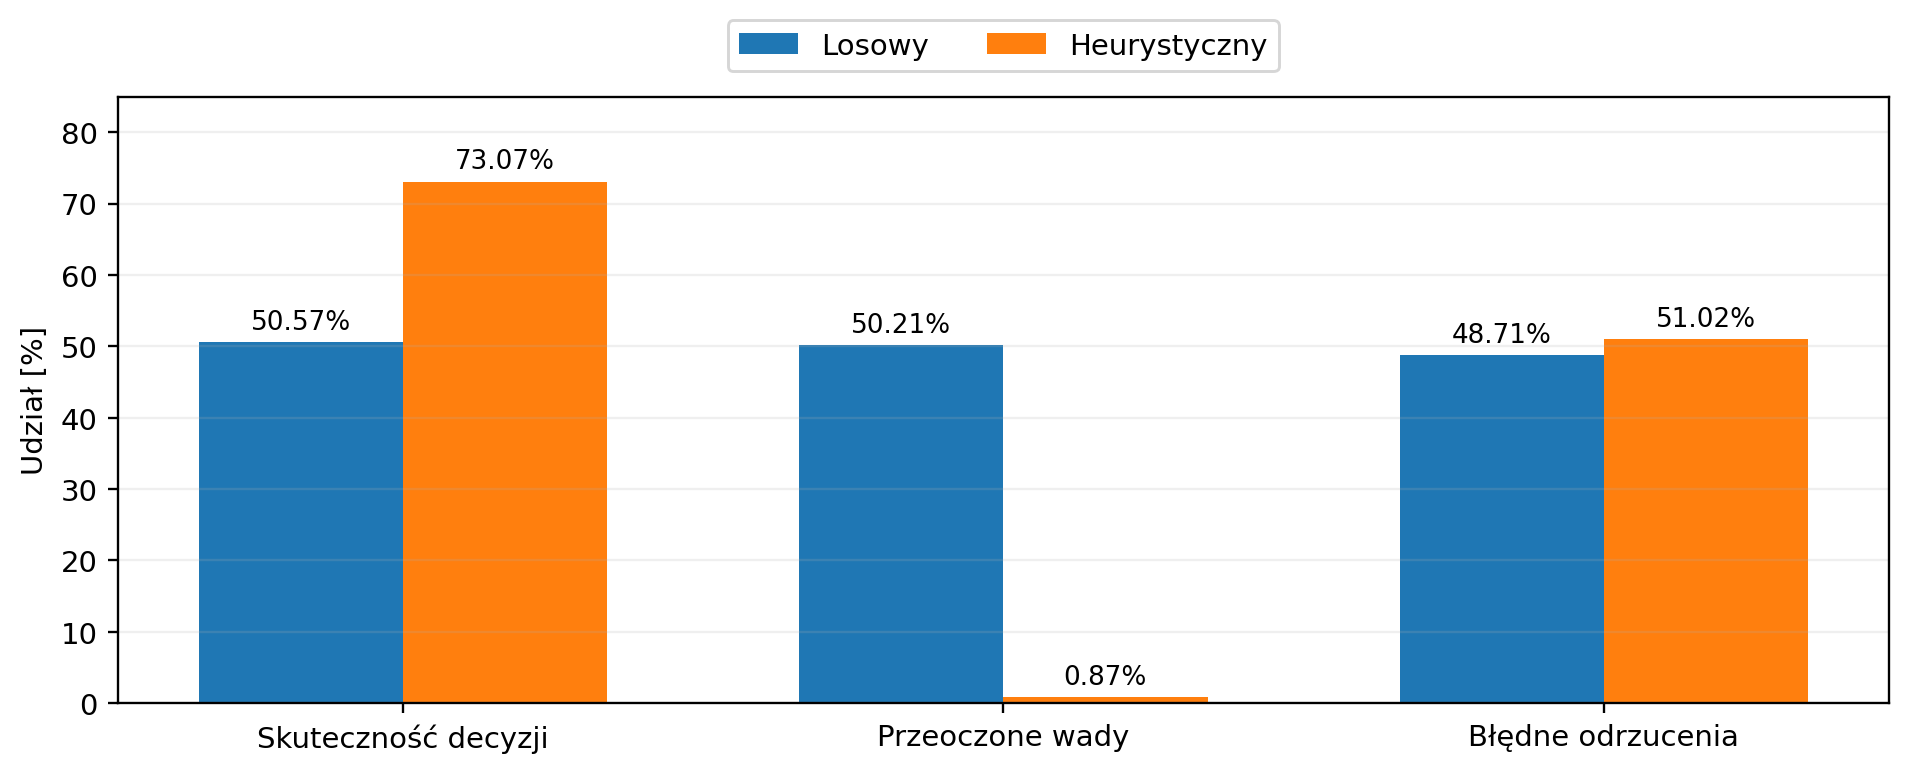
\includegraphics[width=0.94\textwidth]{figures/baseline_comparison.png}%
  }{\fbox{\parbox{0.85\textwidth}{\centering Wykres E2 znajduje się w pliku\\\texttt{figures/baseline\_comparison.png}}}}
  \caption{Wyniki bazowych strategii po 1000 epizodów. Współczynniki przeoczonych wad i błędnych odrzuceń mają różne mianowniki, zgodne z opisem metryk.}
  \label{fig:baselines-e2}
\end{figure}

Dla obu agentów wygenerowano 4804 produkty wadliwe i 5196 poprawnych. Agent losowy poprawnie sklasyfikował 5057 z 10\,000 produktów, przeoczył 2412 wad i odrzucił 2531 produktów poprawnych; wykorzystał w sumie 3095 dodatkowych inspekcji. Agent heurystyczny poprawnie sklasyfikował 7307 z 10\,000 produktów, przeoczył 42 wady i błędnie odrzucił 2651 produktów poprawnych; wykorzystał 1781 dodatkowych inspekcji.

Dla obu wariantów odtworzono zgodność rozmiarów danych: plik szczegółowy zawiera 2000 wierszy (po jednym na epizod), a każdy epizod obejmuje dziesięć decyzji końcowych. Nie stwierdzono przekroczenia budżetu czterech inspekcji w danych z eksperymentu.

\subsection{Wyniki testów programu}

W przeprowadzonym uruchomieniu polecenia \texttt{python -m pytest tests -v} uzyskano wynik \textbf{18 passed}. Testy obejmowały zarówno standardowe działanie środowiska, jak i sytuacje graniczne: zerowy budżet, jednoelementową partię, nielegalne działanie oraz wszystkie przypadki przydzielania nagród.

\section{Analiza i wnioski}

W aktualnym modelu agent heurystyczny uzyskał średni zwrot o \(40{,}884\) punktu wyższy niż agent losowy i zwiększył skuteczność decyzji o \(22{,}50\) punktu procentowego. Jednocześnie zużywał przeciętnie mniej zasobów dodatkowej kontroli (1,781 wobec 3,095 na partię).

Najbardziej widoczną korzyścią heurystyki jest ograniczenie akceptacji wadliwych płytek: odsetek przeoczonych wad zmniejszył się z 50,21\% do 0,87\%. Uzyskano to jednak kosztem dużej liczby odrzuceń poprawnych produktów: 51,02\% wobec 48,71\% dla agenta losowego. Wynika to między innymi ze strategii automatycznego odrzucania przy kategorii wysokiego ryzyka oraz z niedoskonałości podstawowego skanera. W szczególności zakłócenie pomiaru otworu albo pęknięcia z wartości 0 do 1 prowadzi już do wysokiego umownego ryzyka, choć rzeczywista płytka może być prawidłowa.

\textbf{Wniosek E2:} środowisko tworzy sensowny problem decyzyjny o ograniczonym zasobie informacji. Prosta heurystyka przewyższa decyzje losowe, ale nie zapewnia optymalnego bilansu błędów i kosztów. Uzasadnia to dalsze eksperymenty nad algorytmem Q-learning, którego celem będzie wyuczenie polityki lepiej wykorzystującej budżet w całym epizodzie. Nie przesądza to jednak, że algorytm uczący się okaże się lepszy -- wymaga to empirycznej weryfikacji w E3.

\section{Instrukcja uruchomienia}

Do odtworzenia etapu E2 potrzebne są Python 3.12 oraz Git.\par\noindent Biblioteki projektu wymienia plik \texttt{requirements.txt}.\par\noindent Po sklonowaniu publicznego repozytorium należy wykonać w terminalu PowerShell:
\begin{verbatim}
git clone https://github.com/KciamiK/DefectDecision-RL.git
cd DefectDecision-RL
py -3.12 -m venv .venv
.\.venv\Scripts\Activate.ps1
python -m pip install -r requirements.txt
\end{verbatim}

Jeżeli lokalne zasady PowerShell blokują aktywację, można w \emph{bieżącej sesji} wykonać \texttt{Set-ExecutionPolicy -Scope Process -ExecutionPolicy Bypass} i ponowić aktywację. Nie ma potrzeby zmiany globalnych ustawień systemu.

\begin{verbatim}
python src\quality_env.py
python src\random_agent.py
python src\heuristic_agent.py
python experiments\compare_baselines.py
python -m pytest tests -v
\end{verbatim}

Pierwsze trzy polecenia uruchamiają demonstracje, czwarte odtwarza eksperyment z 1000 epizodów na agenta i zapisuje pliki CSV w katalogu \texttt{results/}, a ostatnie uruchamia 18 przypadków testowych. Odwzorowanie wyników wymaga niezmienionego kodu generatora, konfiguracji oraz ziaren losowych podanych w skrypcie.

\section{Wsparcie AI}

W trakcie realizacji E1 i E2 wykorzystywano \textbf{ChatGPT (model GPT-6)} do konsultowania formalizacji problemu, przygotowania i wyjaśniania kodu Pythona, projektowania testów, interpretacji wyników oraz redakcji dokumentacji LaTeX. Wsparcie to było elementem procesu projektowego, a nie samodzielnym potwierdzeniem poprawności programu. Kod został uruchomiony lokalnie, a testy i eksperymenty zweryfikowano na wynikach z terminala i plikach CSV.

\begin{center}
\small
\renewcommand{\arraystretch}{1.2}
\begin{tabular}{p{0.23\textwidth}p{0.23\textwidth}p{0.43\textwidth}}
\toprule
Okres & Narzędzie & Zastosowanie \\
\midrule
5--7 XI 2026 & ChatGPT / GPT-6 & Pomoc przy strukturze repozytorium, modelu produktu, skanerach, środowisku i testach E2 \\
8 XI 2026 & ChatGPT / GPT-6 & Agenci bazowi, skrypt eksperymentów, interpretacja wyników, dokumentowanie E2 \\
\bottomrule
\end{tabular}
\end{center}

\noindent\textbf{Dokumentacja transkryptów:} należy przed oddaniem zachować pełną historię rozmów ze wskazaniem dat i modelu, a gdy narzędzie umożliwia udostępnienie rozmowy -- dołączyć do repozytorium lub raportu rzeczywisty link do jej udostępnienia. Linku nie wpisano automatycznie, ponieważ nie został przekazany.

\noindent\textbf{Weryfikacja:} samodzielna kontrola uruchamiania skryptów, wykonanie 18 testów, odczyt wyników dwóch strategii bazowych oraz decyzje o dalszym zakresie implementacji pozostają odpowiedzialnością autora projektu. Opis wsparcia AI powinien zostać uzupełniony, jeżeli w dalszych etapach pojawią się kolejne sesje lub narzędzia.

\section{Literatura}

W tej sekcji należy wskazać wykorzystane źródła: książki, artykuły naukowe, dokumentację bibliotek, materiały wykładowe oraz inne źródła użyte podczas pracy nad projektem.

\begin{thebibliography}{9}
\bibitem{sutton_barto}
R. S. Sutton, A. G. Barto, \textit{Reinforcement Learning: An Introduction}, 2nd ed., MIT Press, 2018.
\end{thebibliography}

\end{document}
